% It’s Time to Learn drawing Petri Nets in TikZ!
% Concurent processes with mutual resources
% Latexdraw.com
% 17/02/2021, 23:00

\documentclass[border = 0.2cm]{standalone}
\usepackage{tikz}

\usetikzlibrary{decorations.markings,positioning,petri}

\begin{document}

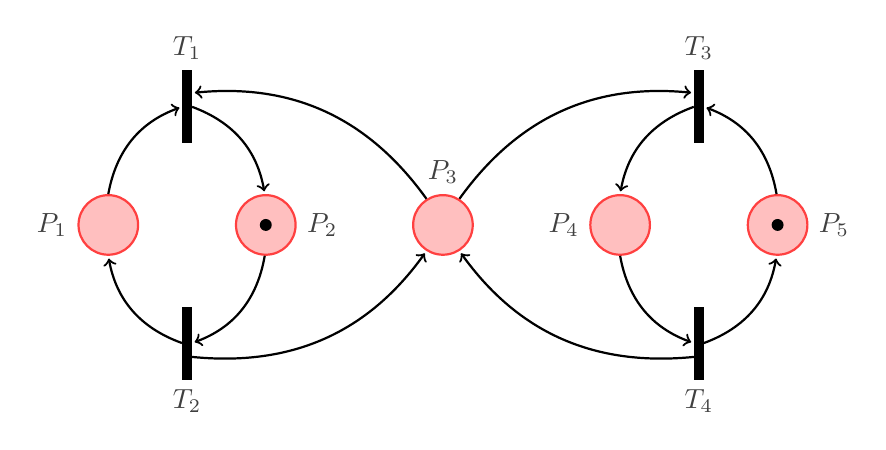
\begin{tikzpicture}[thick,
	node distance=2cm,
	on grid,
	every transition/.style={fill=black,minimum width=.1cm, minimum height=0.9cm},
	every place/.style={fill=red!25,draw=red!75},
	every label/.style={black!75}]

% Places
\node[place,
	label=left:$P_1$] (place1) {};

\node[place,
	right=of place1,
	tokens=1,
	label=right:$P_2$] (place2) {};

\node[place,
	right= 2.25cm of place2,
	label=$P_3$] (place3) {};

\node[place,
	right= 2.25cm of place3,
	label=left:$P_4$] (place4) {};

\node[place,
	right=of place4,
	tokens=1,
	label=right:$P_5$] (place5) {};

% Transitions
\node[transition,
	above left=1.5cm and 1cm of place2,
	label=$T_1$] (T1) {};

\node[transition,
	below left=1.5cm and 1cm of place2,
	label=below:$T_2$] (T2) {};

\node[transition,
	above right=1.5cm and 1cm of place4,
	label=$T_3$] (T3) {};

\node[transition,
	below right=1.5cm and 1cm of place4,
	label=below:$T_4$] (T4) {};

% connections
\draw (T1.east) edge[bend left,post] (place2)
	(place2) edge[bend left,post] (T2.east)
	(T2.west) edge[bend left,post] (place1.south)
	(place1.north) edge[bend left,post] (T1.west);

\draw (T2.-70) edge[bend right,post] (place3)
	(place3)edge[bend right,post] (T1.70);

\draw (T3.east) edge[bend left,pre] (place5) 
	(place5) edge[bend left,pre] (T4.east)
	(T4.west) edge[bend left,pre] (place4.south)
	(place4.north) edge[bend left,pre] (T3.west);

\draw (T4.250) edge[bend left,post] (place3)
	(place3)edge[bend left,post] (T3.110) ;

\end{tikzpicture}

\end{document}
